\documentclass[12pt,a4paper]{report}

% --- Paquets standards ---
\usepackage[utf8]{inputenc}
\usepackage[T1]{fontenc}
\usepackage[french]{babel}
\usepackage{graphicx}
\usepackage{geometry}
\usepackage{xcolor}
\usepackage{hyperref}
\usepackage{amsmath}
\usepackage{amssymb}
\usepackage{booktabs}
\usepackage{float}
\usepackage{caption}
\usepackage{titlesec}
\usepackage{setspace}
\usepackage{fancyhdr}

% --- Configuration des marges ---
\geometry{top=2.5cm, bottom=2.5cm, left=2.5cm, right=2.5cm}

% --- Couleurs ---
\definecolor{sentinelblue}{RGB}{30, 64, 175}
\definecolor{sentinelred}{RGB}{185, 28, 28}

% --- Configuration des liens ---
\hypersetup{
    colorlinks=true,
    linkcolor=sentinelblue,
    filecolor=magenta,      
    urlcolor=cyan,
    citecolor=sentinelblue,
}

% --- Styles des titres ---
\titleformat{\chapter}[display]
  {\normalfont\bfseries\color{sentinelblue}\Huge}{\chaptertitlename\ \thechapter}{20pt}{\Huge}

% --- En-tête et Pied de page ---
\pagestyle{fancy}
\fancyhf{}
\lhead{AirSentinel Cameroun -- IndabaX 2026}
\rhead{DPA Green Tech}
\cfoot{\thepage}

% --- Informations du document ---
\title{
    
\includegraphics[width=0.3\textwidth]{../assets/logo.jpg} \\ \vspace{1cm}
    \textbf{\Huge AirSentinel Cameroun} \\ \vspace{0.5cm}
    {\large Système intelligent de surveillance et de prédiction de la qualité de l'air pour 40 villes camerounaises}
}
\author{
    \textbf{Équipe DPA Green Tech} \\
    BODEHOU Sabine (ISSEA Yaoundé) \\
    FANKAM Marc Aurel (ISSEA Yaoundé) \\
    PEURBAR RIMBAR Firmin (ISSEA Yaoundé) \\
    FOFACK ALEMDJOU Henri Joël (ENSP Yaoundé)
}
\date{Hackathon IndabaX Cameroon 2026}

\begin{document}

\maketitle

\begin{abstract}
La pollution atmosphérique constitue un défi majeur de santé publique au Cameroun. AirSentinel est une solution intégrée de \textit{Data Science} visant à pallier l'absence de réseau de surveillance en temps réel. Notre approche combine un pipeline ETL automatisé collectant les données de 40 villes, un modèle prédictif hybride (Random Forest + ARIMA) atteignant un $R^2$ de 0.893, et un Indice de Risque Sanitaire (IRS) robuste calculé par Analyse en Composantes Principales (ACP). Le système est rendu accessible via une Progressive Web App (PWA) ultra-légère et un dashboard analytique détaillé pour les décideurs.
\end{abstract}

\tableofcontents

\chapter{Introduction}
\section{Contexte et Enjeux}
Selon les estimations, plus de 90\% des villes camerounaises dépassent les seuils recommandés par l'OMS pour les particules fines PM2.5. L'exposition prolongée à ces polluants est corrélée à une augmentation des pathologies respiratoires et cardiovasculaires.

\section{Problématique}
Il existe un manque critique de stations de mesure physiques et de systèmes d'alerte précoce au Cameroun. Les populations et les autorités sanitaires ne disposent pas d'informations exploitables pour réduire l'exposition lors des épisodes critiques (ex: Harmattan, feux de brousse).

\section{Objectifs du Projet}
L'objectif d'AirSentinel est de fournir un système de décision sanitaire basé sur l'IA capable de :
\begin{itemize}
    \item Surveiller en continu les indicateurs climatiques et toxiques.
    \item Prédire la concentration de PM2.5 à un horizon de 72 heures.
    \item Offrir des recommandations sanitaires personnalisées basées sur les directives de l'OMS 2021.
\end{itemize}

\chapter{Méthodologie}
\section{Acquisition et Traitement des Données}
Le projet exploite l'API Open-Meteo pour collecter les chroniques temporelles horaires de 40 villes représentatives des 10 régions du Cameroun. Le dataset final comprend plus de 50 000 observations intégrant : température, humidité, vitesse du vent, CO, NO2, O3, et PM2.5.

\section{Modélisation Hybride}
Nous avons implémenté un modèle combiné pour capturer à la fois les corrélations structurelles et la saisonnalité climatique camerounaise :
\begin{enumerate}
    \item \textbf{Base de Régression :} Un modèle Random Forest optimisé pour traiter les interactions non linéaires entre les variables météo et la concentration de polluants.
    \item \textbf{Ajustement Temporel (ARIMA) :} Un correcteur de séries temporelles segmenté par zone INS (Équatoriale, Soudanienne, Soudano-Sahélienne).
\end{enumerate}

\section{Indice de Risque Sanitaire (IRS)}
Plutôt que de se limiter au seul PM2.5, nous calculons un IRS multidimensionnel par \textbf{Analyse en Composantes Principales (ACP)}. L'ACP sur 5 variables (PM2.5, Dust, CO, UV, O3) permet d'extraire un score unique normalisé [0, 1] reflétant le risque global de pollution.

\chapter{Résultats et Analyse}
\section{Performances Prédictives}
Le modèle AirSentinel surpasse significativement les baselines statistiques classiques.
\begin{table}[H]
\centering
\begin{tabular}{lc}
\toprule
Métrique & Valeur Obtenue \\
\midrule
$R^2$ (Coefficient de détermination) & \textbf{0.893} \\
MAE (Erreur Absolue Moyenne) & 3.456 $\mu g/m^3$ \\
Taux de détection des pics ($> 35 \mu g/m^3$) & 79.6\% \\
\bottomrule
\end{tabular}
\caption{Mesures de performance sur le jeu de test 2025.}
\end{table}

\section{Visualisation de l'ajustement}
La figure \ref{fig:predict} montre la capacité du modèle à suivre les dynamiques réelles du PM2.5, notamment lors des pics de février 2025.
\begin{figure}[H]
    \centering
    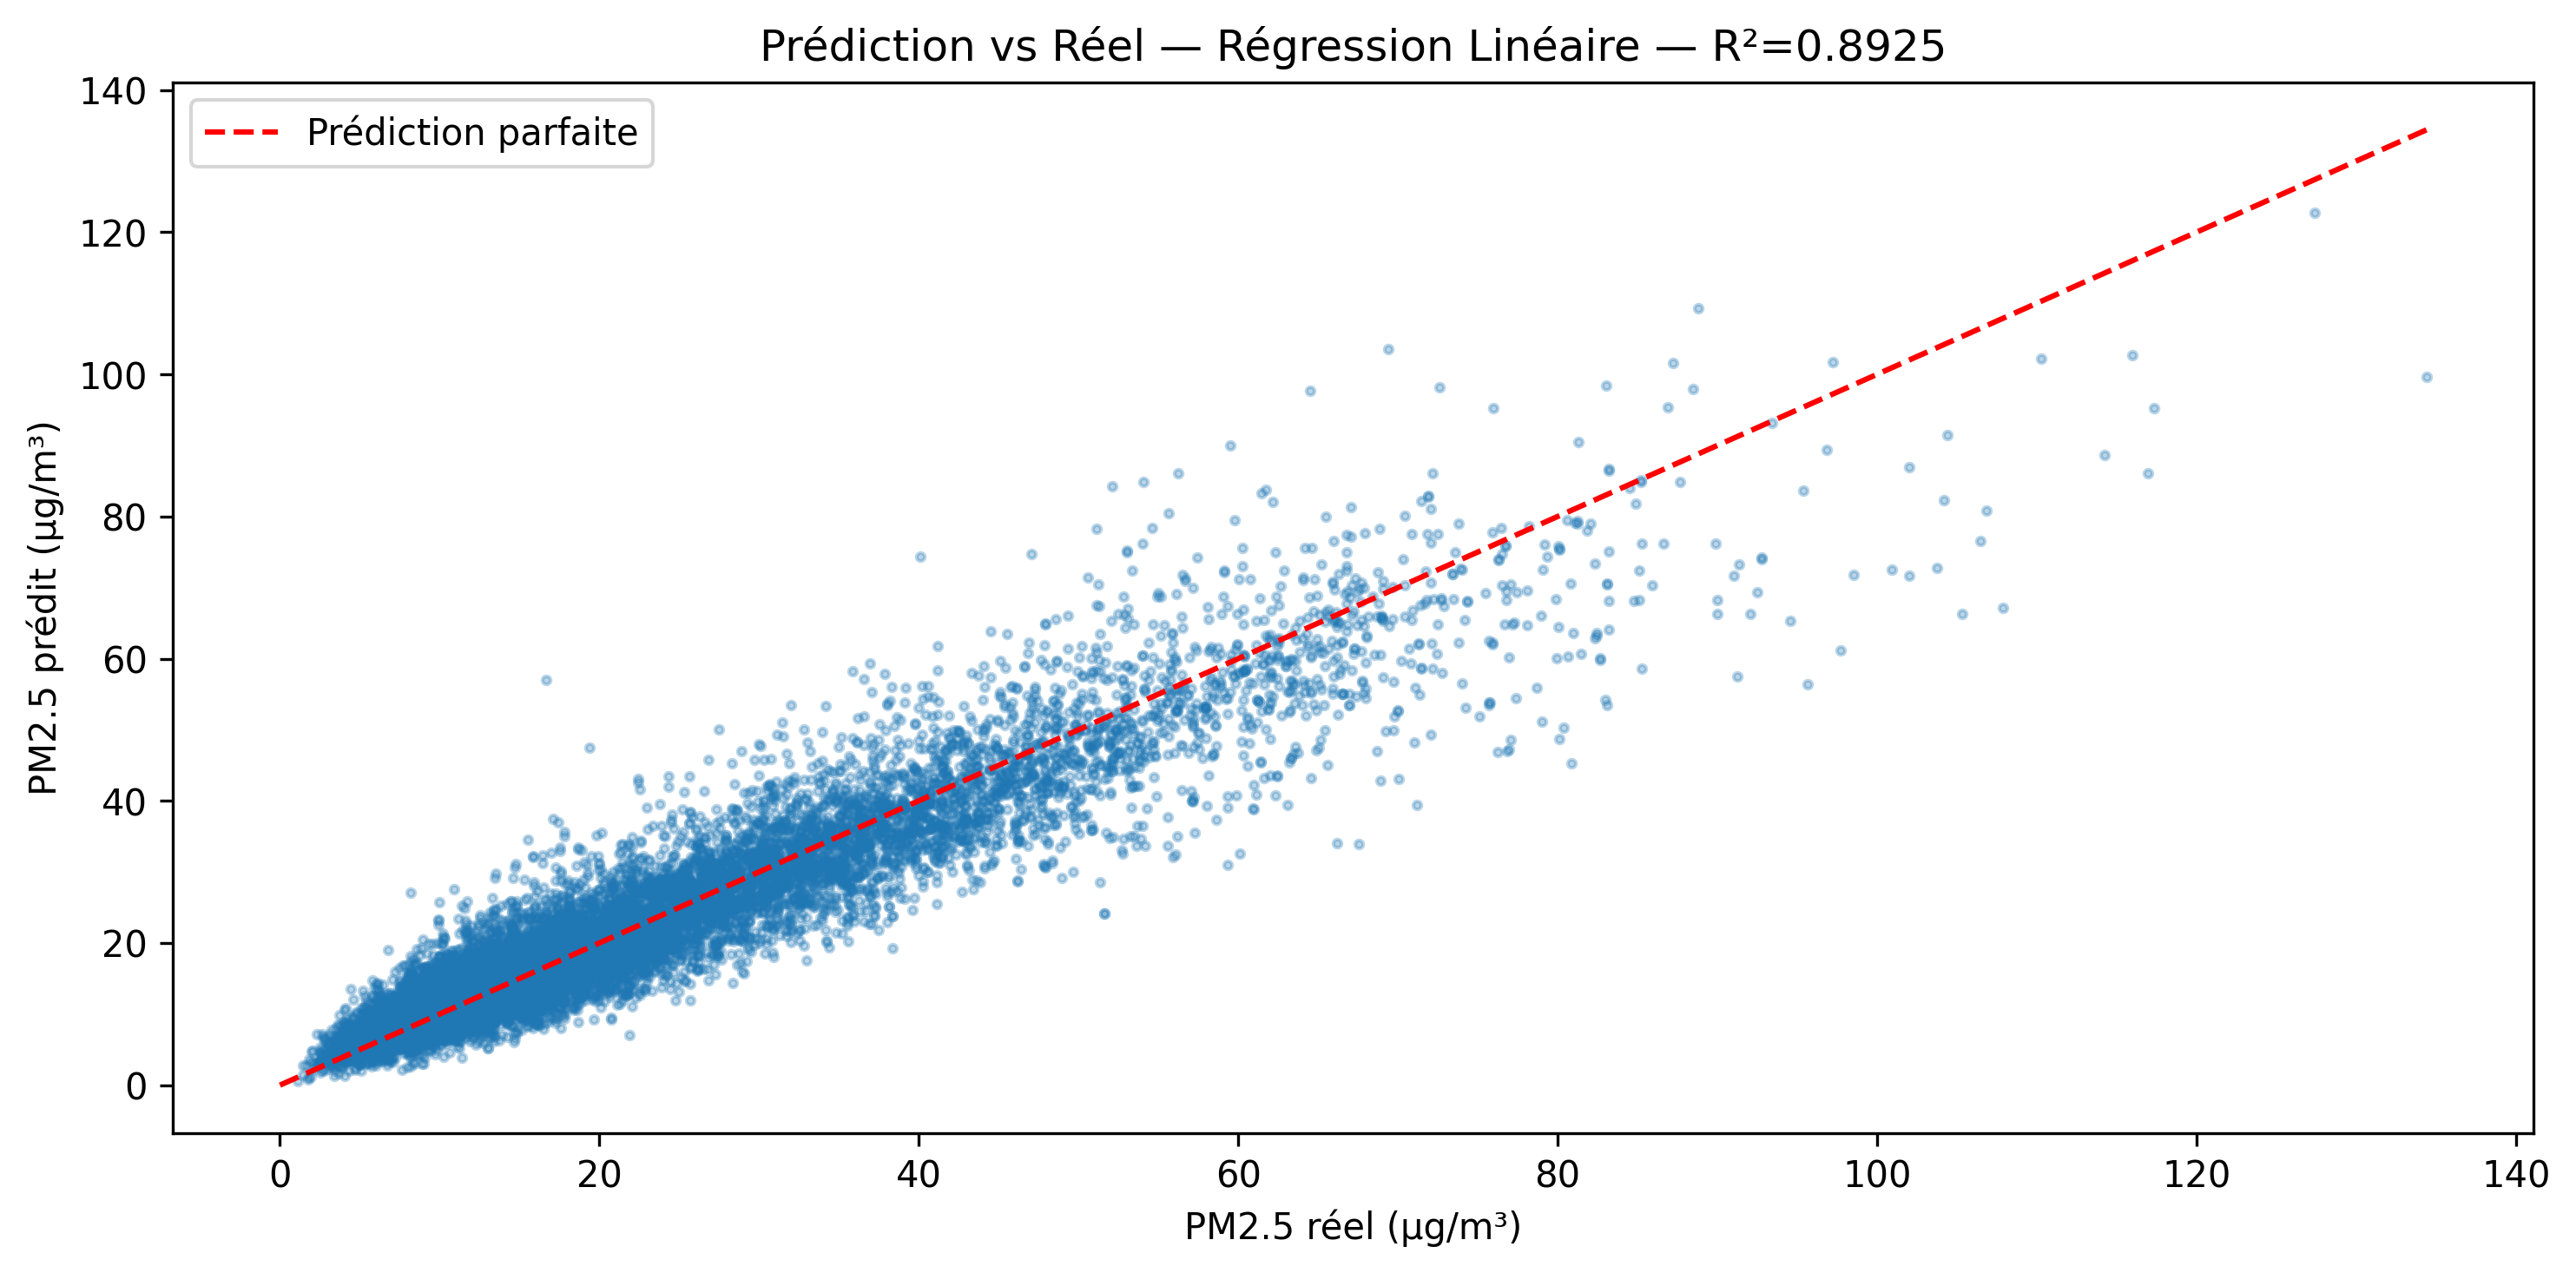
\includegraphics[width=0.8\textwidth]{../graphiques/prediction_vs_reel.png}
    \caption{Comparaison entre PM2.5 réel et prédit.}
    \label{fig:predict}
\end{figure}

\section{Analyse SHAP et Explicabilité}
Grâce à la méthode SHAP \cite{shap2017}, nous avons identifié les facteurs aggravants par zone. Dans le Grand Nord, la \textit{Dust} (poussière saharienne) est le prédicteur dominant, tandis que dans le Littoral, l'humidité et le CO (traceur industriel/feux) sont prépondérants.

\begin{figure}[H]
    \centering
    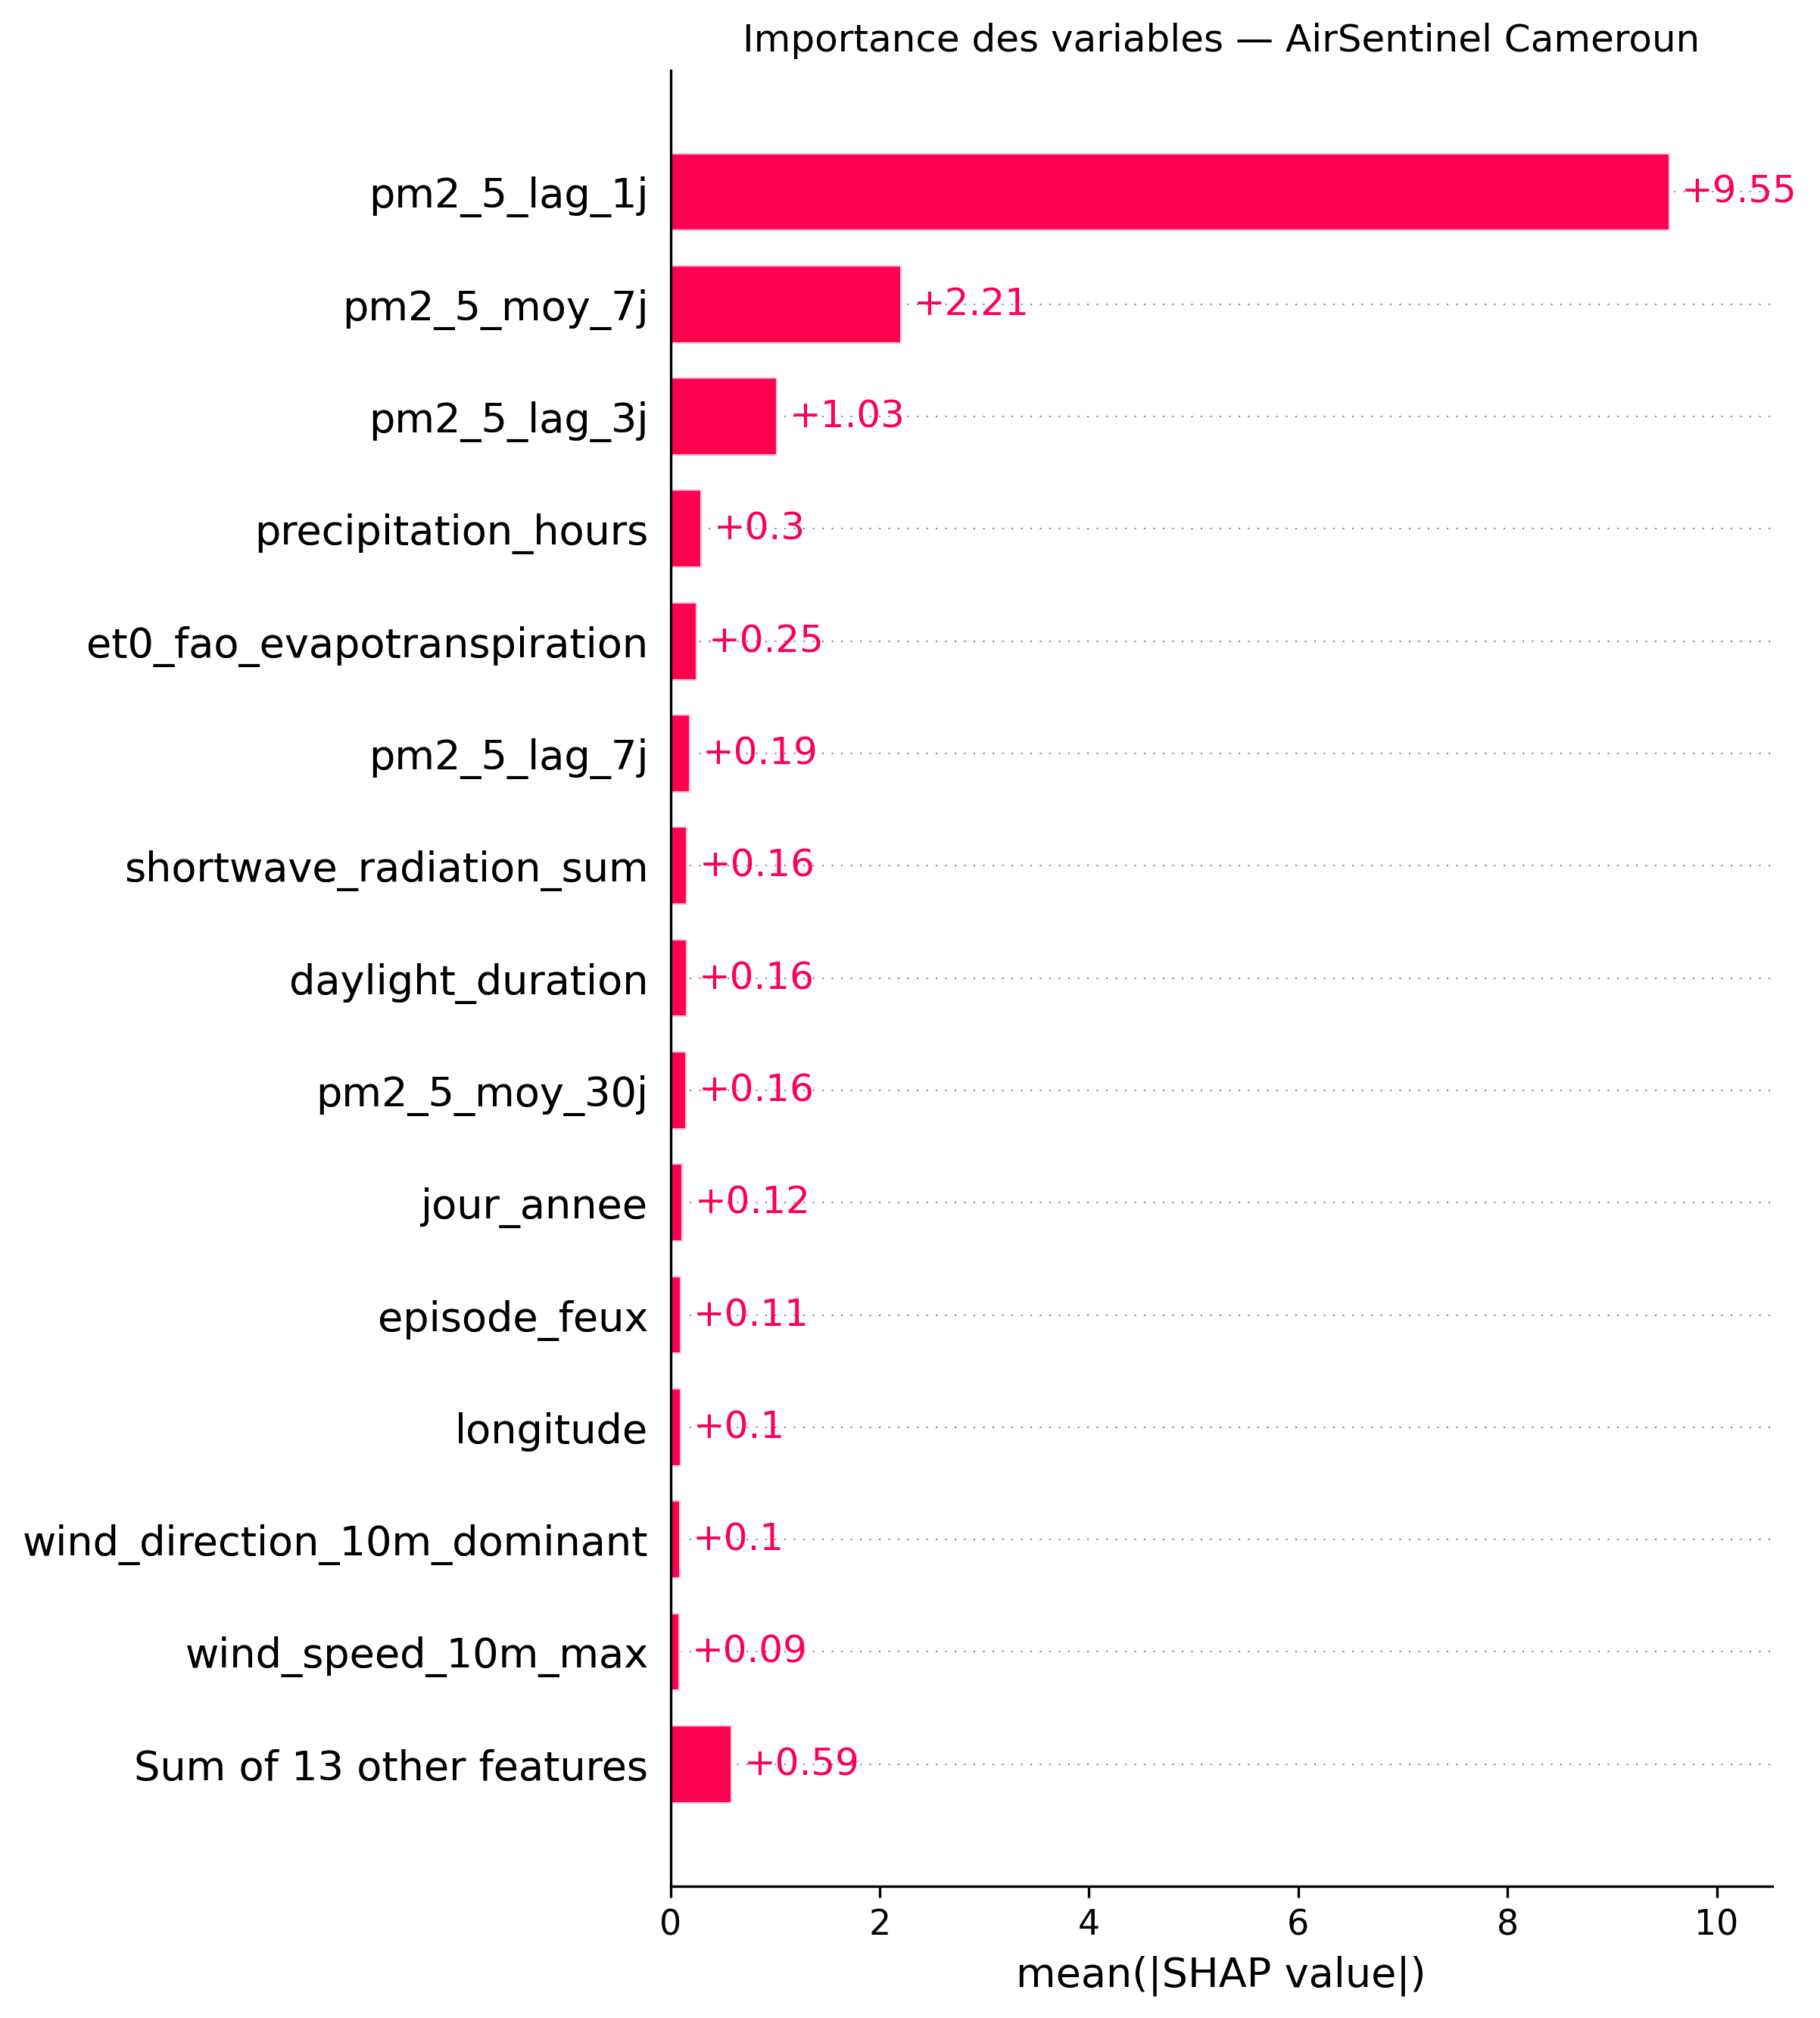
\includegraphics[width=0.8\textwidth]{../graphiques/shap_importance.png}
    \caption{Importance globale des variables via SHAP.}
\end{figure}

\chapter{La Solution AirSentinel}
\section{Architecture Cloud}
Le backend FastAPI est conteneurisé et déployé sur Render. L'automatisation est assurée par GitHub Actions qui déclenche la mise à jour quotidienne à 03:00 UTC.

\section{Interface Mobile (PWA)}
L'application mobile a été conçue pour être "Offline-First". Elle permet à un citoyen de consulter l'indice de risque de sa ville même avec une connexion instable.
% Note : Insérer ici une capture d'écran du téléphone
% \includegraphics[width=0.4\textwidth]{../assets/screenshots/mobile_app.png}

\section{Dashboard Analytique}
Destiné aux chercheurs et maires, le dashboard Streamlit permet une exploration profonde (filtrage par région, rapports PDF, simulation météo).

\chapter{Conclusion}
AirSentinel démontre que l'IA, couplée à des données \textit{Open Access}, peut transformer la surveillance environnementale au Cameroun avec un budget de fonctionnement quasi-nul. Notre modèle hybride offre une précision suffisante pour une alerte sanitaire fiable. Les perspectives incluent l'intégration de données satellites haute résolution et le déploiement de capteurs LoRaWAN pour valider nos modèles au sol.

\bibliographystyle{unsrt}
\bibliography{references}

\end{document}
